Vi fjerner strap S2.

\subsection{Oppg 2a}
La B være ’høy’ - (ikke trykk på knappen) \\
Ved hvilken spenning på A skifter utgangen tilstand til lav? Forklar hvorfor.
\\\\
Vi måler utgangsspenningen mens vi justerer spenningen over A fra 5V og nedover.
Utgangsspenningen holder seg på ca 21mV lenge til den såvidt begynner å stige.
Den stiger svakt i mV skala til den plutselig hopper opp til 1V.
Der er spenningen over A ~1.1V.

\paragraph{Forklaring} \mbox{} \\
For at det skal gå strøm gjennom transistoren må strømmen gjennom D3, D4 og BE,
tilsammen må spenningen være $0.6 + 0.6 + 0.6 = 1.8$.
Vi måtte spille A til 1.1V som sammen med dioden er $1.1 + 0.6 = 1.7$.
Fordi diodene ikke er perfekte vil det gå strøm litt før ideelt sett,
altså er 1.7 nok til å få strøm i kretsen.



\subsection{Oppg 2b}
Tegn opp sammenhengen mellom spenningen over A og 
Vut.  
Pass på å få med med noen ekstra verdier rundt overgangen 
fra ’høy’ til ’lav’.
\begin{figure}[H]
  \caption{Sammenheng mellom spenning over A og spenning ut.}
  \centering
    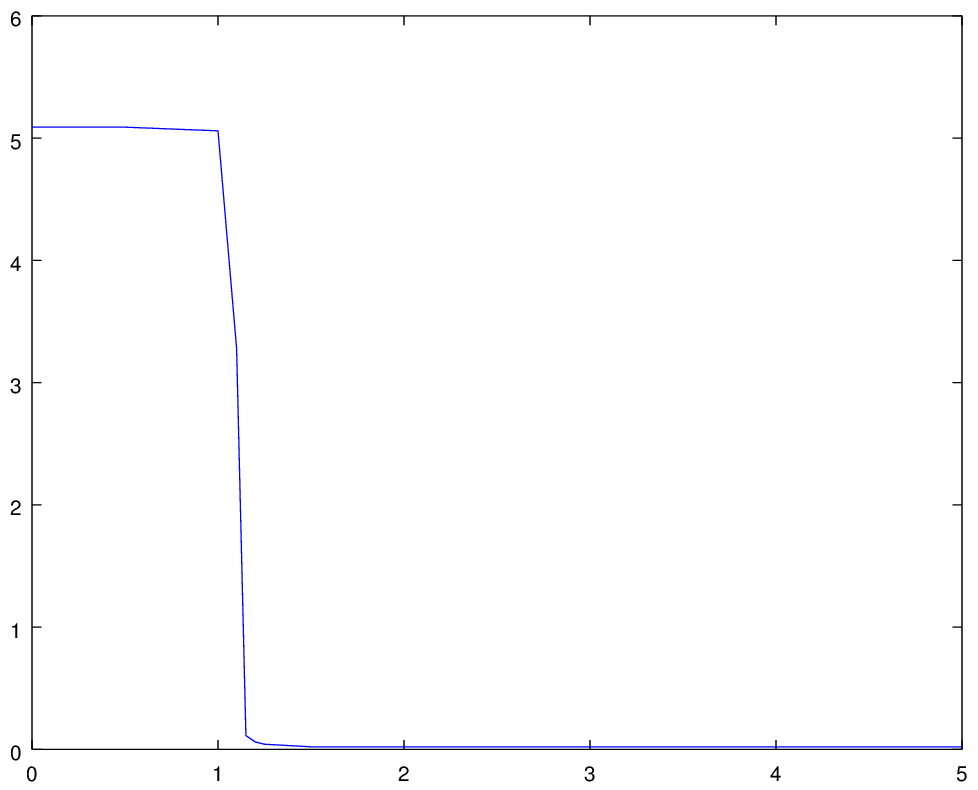
\includegraphics[width=\textwidth]{2b.png}
\end{figure}

\begin{figure}[H]
  \lstinputlisting{2b.matlab}
  \caption{Koden tilhørende plot.}
\end{figure}
